% Compile with pdflatex
% Gemini theme — fork of https://github.com/anishathalye/gemini

\documentclass[final]{beamer}

% ====================
% Packages
% ====================

\usepackage[T1]{fontenc}
\usepackage{lmodern}
\usepackage[size=custom,width=91.44,height=60.96,scale=0.85]{beamerposter}
\usetheme{gemini}
\usecolortheme{stanford}
\usepackage{graphicx}
\usepackage{booktabs}
\usepackage{tikz}
\usepackage{amsmath}
\usepackage{amssymb}

% Manual citations (to avoid bibliography rendering issues)
\newcommand{\citeman}[1]{[#1]}

% ====================
% Lengths
% ====================

\newlength{\sepwidth}
\newlength{\colwidth}
\setlength{\sepwidth}{0.025\paperwidth}
\setlength{\colwidth}{0.3\paperwidth}

\newcommand{\separatorcolumn}{\begin{column}{\sepwidth}\end{column}}

% ====================
% Title
% ====================

\title{SwishNet: Predicting NBA Shot Outcomes with Spatio-Temporal GNNs}

\author{Anthony Argyropoulos}

\institute[shortinst]{Department of Computer Science, Stanford University \quad aargy@stanford.edu}

% ====================
% Footer
% ====================

\footercontent{
  Stanford University \hfill
  Winter 2025--26 \hfill
  aargy@stanford.edu}

% ====================
% Body
% ====================

\begin{document}

\addtobeamertemplate{headline}{}
{
    \begin{tikzpicture}[remember picture,overlay]
      \node [anchor=north east, inner sep=3cm] at ([xshift=0.0cm,yshift=2.5cm]current page.north east)
      {
\includegraphics[height=7.0cm]{stanford_logos/Block_S_2_color.png}};
    \end{tikzpicture}
}

\begin{frame}[t]
\begin{columns}[t]
\separatorcolumn

% ============================================================
% COLUMN 1
% ============================================================
\begin{column}{\colwidth}

  \begin{block}{Predicting}
    NBA shot outcomes are stochastic, but the spatial context surrounding each shot carries predictive signal that tabular features miss. We present \textbf{SwishNet}, predicting make/miss from SportVU tracking data on \textbf{87,147 shots}. The input is a spatio-temporal graph $\mathcal{G}$ built from $(x,y,z)$ positions at shot release and 2--4 preceding snapshots; the output is $\hat{p} \in [0,1]$. We benchmark LR, decision trees, and XGBoost against four GNN operators and 29 HP configs. Our hybrid pipeline (GNN + GMM + XGBoost) achieves \textbf{AUC 0.6551}.
  \end{block}

  \begin{block}{Data, Features \& Graph Construction}
    \textbf{2015--16 NBA SportVU}: $(x,y,z)$ of 10 players + ball at 25\,Hz, 632 games, aligned with play-by-play and 21 per-player stats. \textbf{87,147 shots} (FG\% 45.8\%). GNN: 61K/17K/8.7K; baselines: 5-fold CV.

    \vspace{-1ex}
    \begin{table}
      \centering
      \small
      \begin{tabular}{l l}
        \toprule
        \textbf{Static-38} & \textbf{Velocity-65 (+27)} \\
        \midrule
        Ball-to-rim dist (ft), ball height (ft), angle ($^\circ$) & Ball velocity $(v_x, v_y, v_z)$ (ft/s), speed \\
        3PT flag, shot/game clocks (s), quarter & Launch-angle proxy ($^\circ$) \\
        Teammate distances (4) (ft) & Shooter velocity $(v_x, v_y)$ (ft/s), speed \\
        Defender distances (5) (ft), defs $<$6\,ft & 4 teammate speeds (ft/s) \\
        21 shooter career stats (\%) & 5 defender velocities, closing speeds (ft/s) \\
        \bottomrule
      \end{tabular}
      \vspace{-1ex}
    \end{table}

    \vspace{-1ex}
    \begin{figure}
      \centering
      \begin{minipage}{0.48\linewidth}
        \centering
        
\includegraphics[width=\linewidth]{weights_velocity_lasso.png}
      \end{minipage}\hfill
      \begin{minipage}{0.48\linewidth}
        \centering
        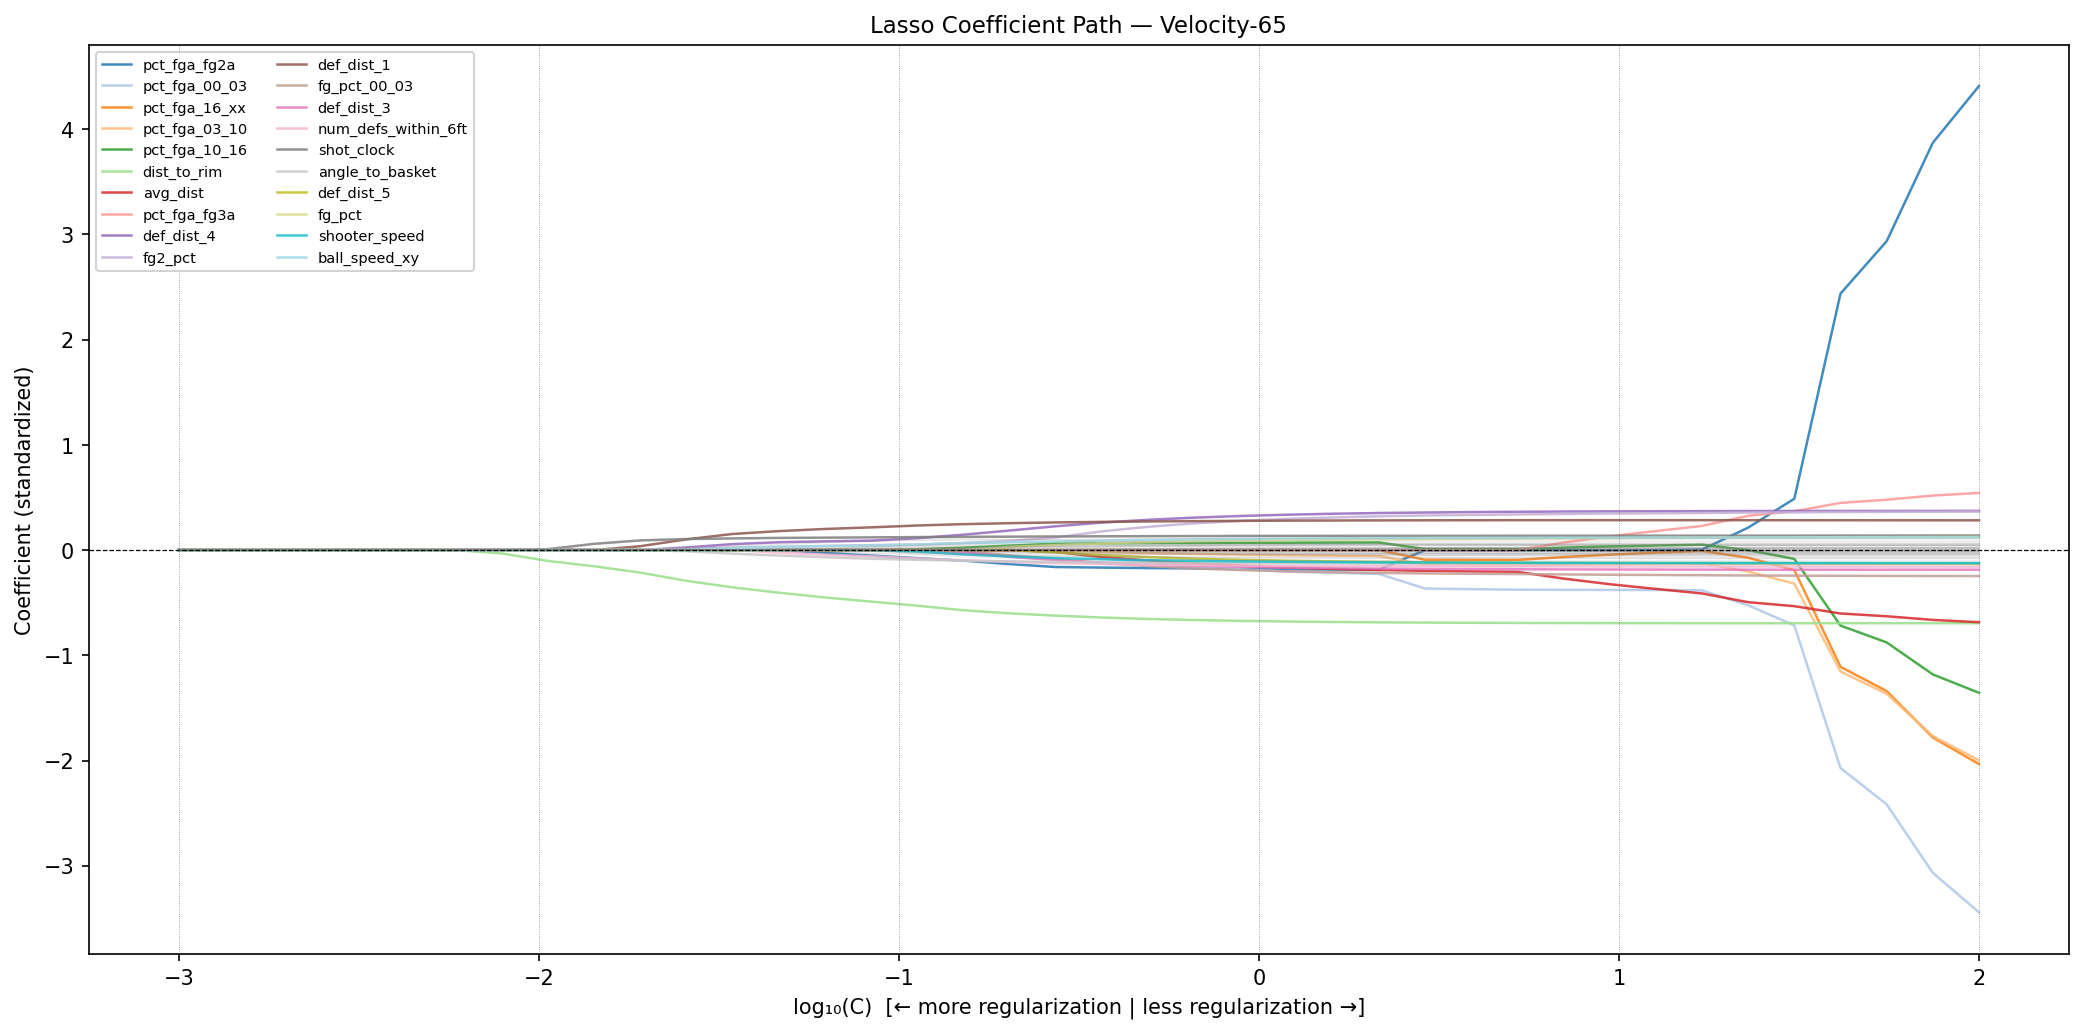
\includegraphics[width=\linewidth]{lasso_path_velocity.png}
      \end{minipage}
      \vspace{-1ex}
      \caption{Left: Top-30 Lasso coefficients. Right: Lasso path vs.\ regularization.}
    \end{figure}
    \vspace{-2ex}

    \heading{Graph}
    A physics-based algorithm scans backward from PBP events to locate the release frame via rim-moment detection and shooter identification.
    Per timestep: 11 fully-connected nodes (5 off + 5 def + ball). Default: 3 snapshots at offsets [3,\,12] frames behind release (0.12\,s and 0.48\,s at 25\,Hz), yielding 33 nodes and ${\sim}$330 edges.
    \vspace{-1ex}

    \begin{minipage}{0.38\linewidth}
      \begin{figure}
        \centering
        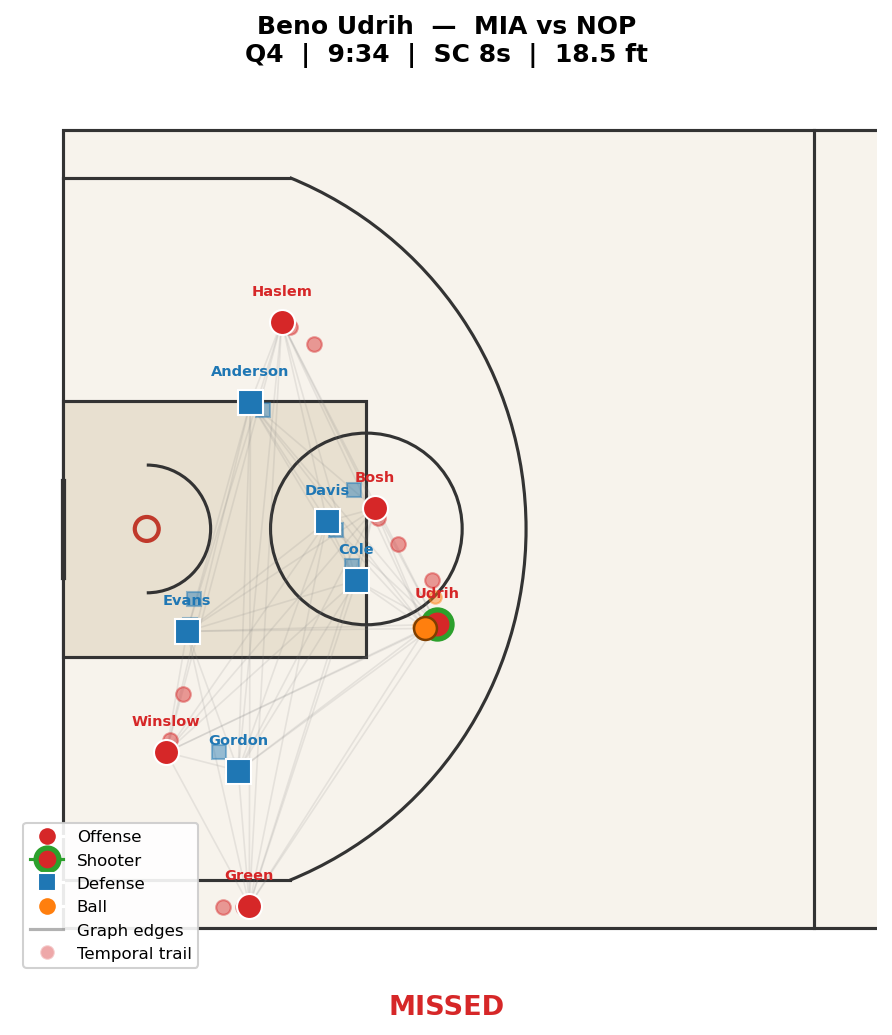
\includegraphics[width=\linewidth,height=6.5cm,keepaspectratio,trim=60 80 60 60,clip]{shot_udrih_missed.png}\\[0.3ex]
        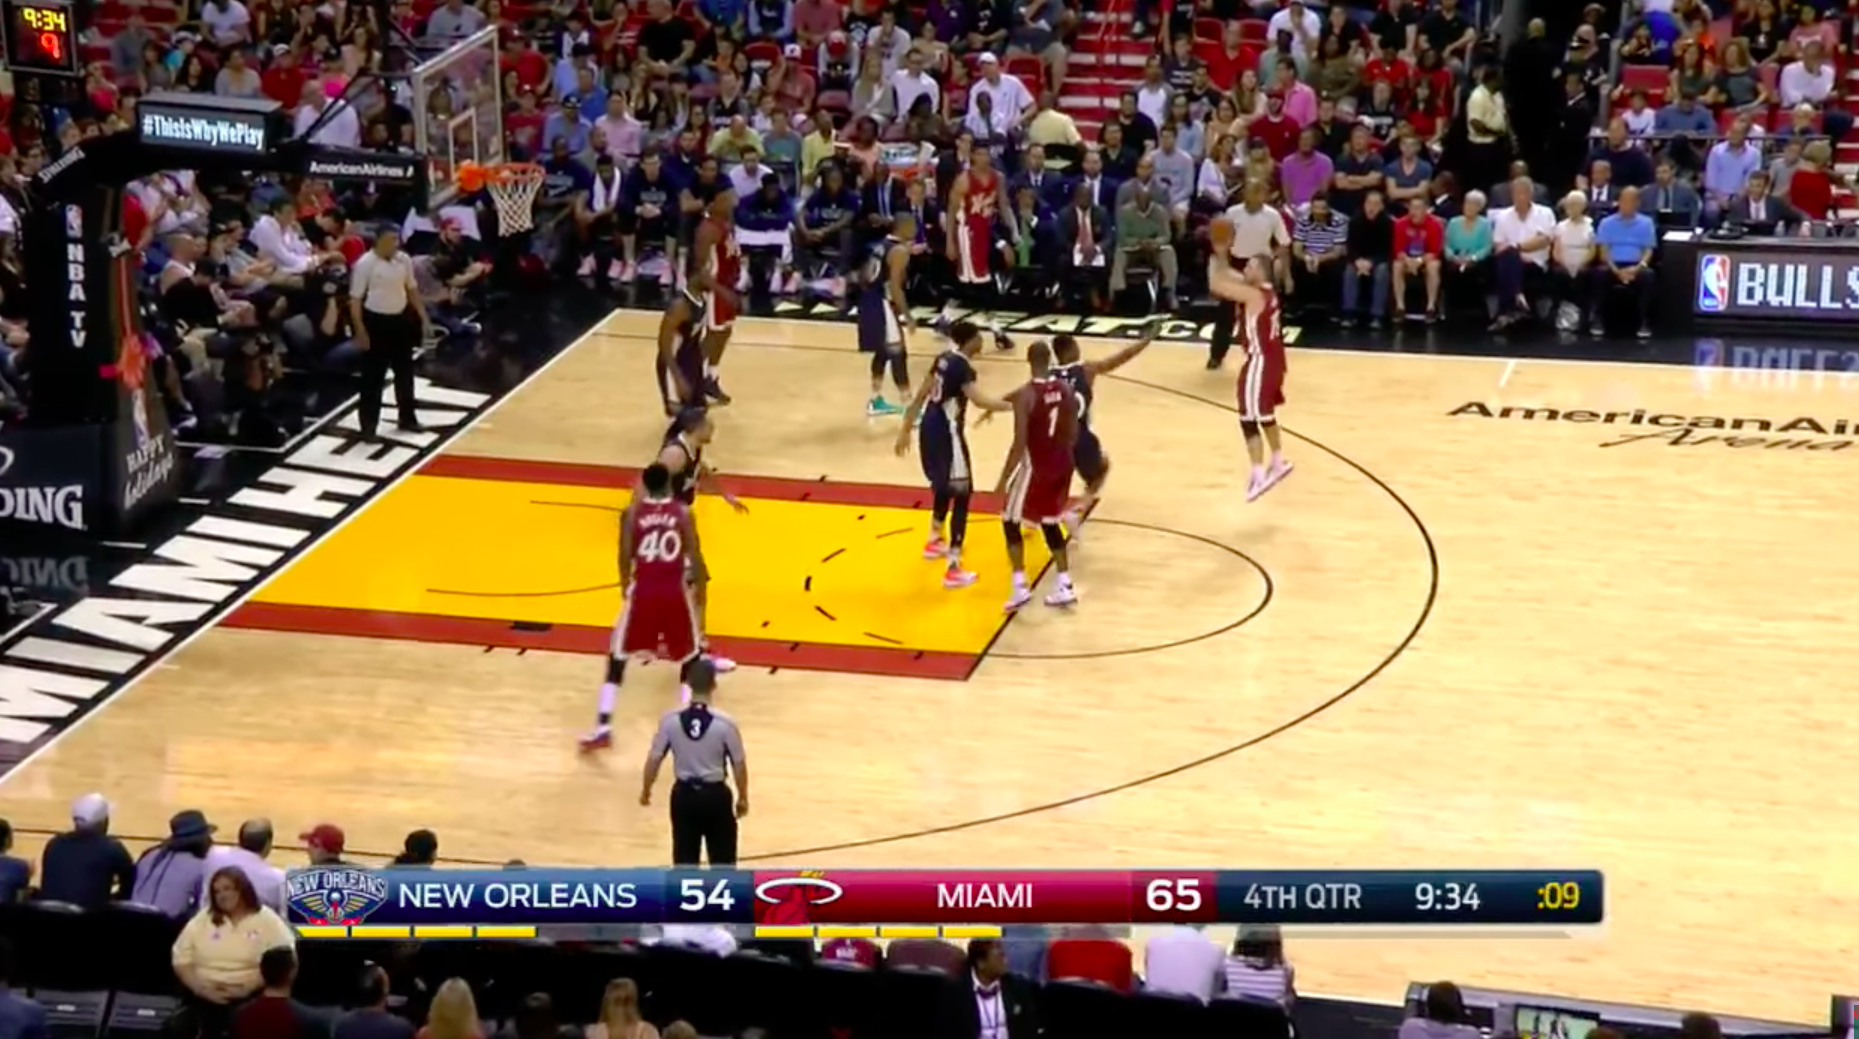
\includegraphics[width=\linewidth,height=3.5cm,keepaspectratio]{udrih_missed.png}
        \vspace{-1ex}
        \caption{Udrih mid-range miss, MIA vs NOP: graph (top) and game footage (bottom).}
      \end{figure}
    \end{minipage}\hfill
    \begin{minipage}{0.58\linewidth}
      \begin{table}
        \centering
        \scriptsize
        \begin{tabular}{l l}
          \toprule
          \multicolumn{2}{c}{\textbf{Node Features (41 per node)}} \\
          \midrule
          $x, y, z$ & Court position (ft) \\
          has\_ball, is\_offense & Binary role flags \\
          is\_player\_node & 1 for players, 0 for ball \\
          dist\_to\_rim, angle\_to\_basket & Geometry (ft, $^\circ$) \\
          dist\_to\_ball\_handler & Spacing (ft) \\
          dist\_to\_3pt\_line & Court zone (ft) \\
          num\_nearby\_defenders & Count within 6\,ft \\
          quarter, game\_clock, shot\_clock & Game state (s) \\
          timestamp & Temporal index (0--2) \\
          position\_encoding (5) & Learnable node ID \\
          player\_stats (21) & Career shooting \% \\
          \midrule
          \multicolumn{2}{c}{\textbf{Edge Features (9 per edge)}} \\
          \midrule
          $\Delta x$, $\Delta y$ & Relative position (ft) \\
          euclidean\_dist & Pairwise distance (ft) \\
          edge\_angle & Bearing ($^\circ$) \\
          type: OO, OD, DD, PB & One-hot relation type \\
          type: TEMPORAL & Temporal link flag \\
          \bottomrule
        \end{tabular}
        \vspace{-1ex}
        \caption{Node and edge feature vectors for each spatio-temporal graph.}
      \end{table}
    \end{minipage}
  \end{block}

\end{column}

\separatorcolumn

% ============================================================
% COLUMN 2
% ============================================================
\begin{column}{\colwidth}

  \begin{block}{Models}

    \heading{Logistic Regression}
    $p(y{=}1 \mid \mathbf{x}) = \sigma(\mathbf{w}^\top\mathbf{x} + b)$ where $\sigma(z) = 1/(1+e^{-z})$. Fit by minimizing cross-entropy with $L_1$ (Lasso) or $L_2$ (Ridge) regularization; strength $C = 1/\lambda$ selected via inner 3-fold CV.

    \heading{XGBoost [1]}
    Additive ensemble $\hat{y}_i = \sum_{t=1}^{T} f_t(\mathbf{x}_i)$, trained by gradient boosting. $T{=}400$ trees, depth$=$4, $\eta{=}0.05$.

    \heading{GATv2Conv [2]}
    Dynamic attention applied \textit{after} concatenation:
    \vspace{-0.8em}
    $$\alpha_{ij} = \frac{\exp(\mathbf{a}^\top \text{LeakyReLU}(\mathbf{W}[\mathbf{h}_i \| \mathbf{h}_j \| \mathbf{e}_{ij}]))}{\sum_{k \in \mathcal{N}(i)} \exp(\mathbf{a}^\top \text{LeakyReLU}(\mathbf{W}[\mathbf{h}_i \| \mathbf{h}_k \| \mathbf{e}_{ik}]))}$$
    \vspace{-0.8em}

    \heading{GINEConv}
    Injective neighborhood aggregation with edge features:
    \vspace{-0.8em}
    $$\mathbf{h}_i' = \text{MLP}\!\Big((1{+}\epsilon)\,\mathbf{h}_i + \sum_{j \in \mathcal{N}(i)} \text{ReLU}(\mathbf{h}_j + \mathbf{e}_{ij})\Big)$$
    \vspace{-0.8em}

    \heading{Temporal GRU Aggregation [3]}
    Per-timestep GATv2/GINE $\to$ mean pool $\to$ $\mathbf{h}_t {\in} \mathbb{R}^{d}$. GRU aggregates the sequence:
    \vspace{-0.8em}
    $$\mathbf{z}_t = \sigma(\mathbf{W}_z[\mathbf{h}_t \| \mathbf{s}_{t-1}]),\quad \mathbf{s}_t = (1{-}\mathbf{z}_t)\odot\mathbf{s}_{t-1} + \mathbf{z}_t\odot\tanh(\mathbf{W}[\mathbf{h}_t \| \mathbf{r}_t{\odot}\mathbf{s}_{t-1}])$$
    \vspace{-0.5em}
    Final $\mathbf{s}_T {\in} \mathbb{R}^{256}$ classified by 3-layer MLP.

    \heading{PCA + Gaussian Mixture Model}
    We reduce 256-dim GRU embeddings via PCA (88.4\% variance in 2 PCs), then fit a GMM ($K{=}10$, BIC-selected):
    \vspace{-0.8em}
    $$p(\mathbf{z}) = \sum_{k=1}^{K} \pi_k \,\mathcal{N}(\mathbf{z};\, \boldsymbol{\mu}_k,\, \boldsymbol{\Sigma}_k)$$
    \vspace{-0.8em}
    Each shot receives a 10-dim soft membership vector $[\gamma_{i,1}, \ldots, \gamma_{i,10}]$.
  \end{block}

  \begin{block}{Hybrid Pipeline: GNN + GMM + XGBoost}
    The GMM recovers 10 NBA shot archetypes \textit{without supervision} from the GNN's latent space. We concatenate the 10-dim soft membership vector with Static-38 features and retrain XGBoost, yielding \textbf{AUC 0.6551}---our best result.
    \vspace{-1ex}
    \begin{figure}
      \centering
      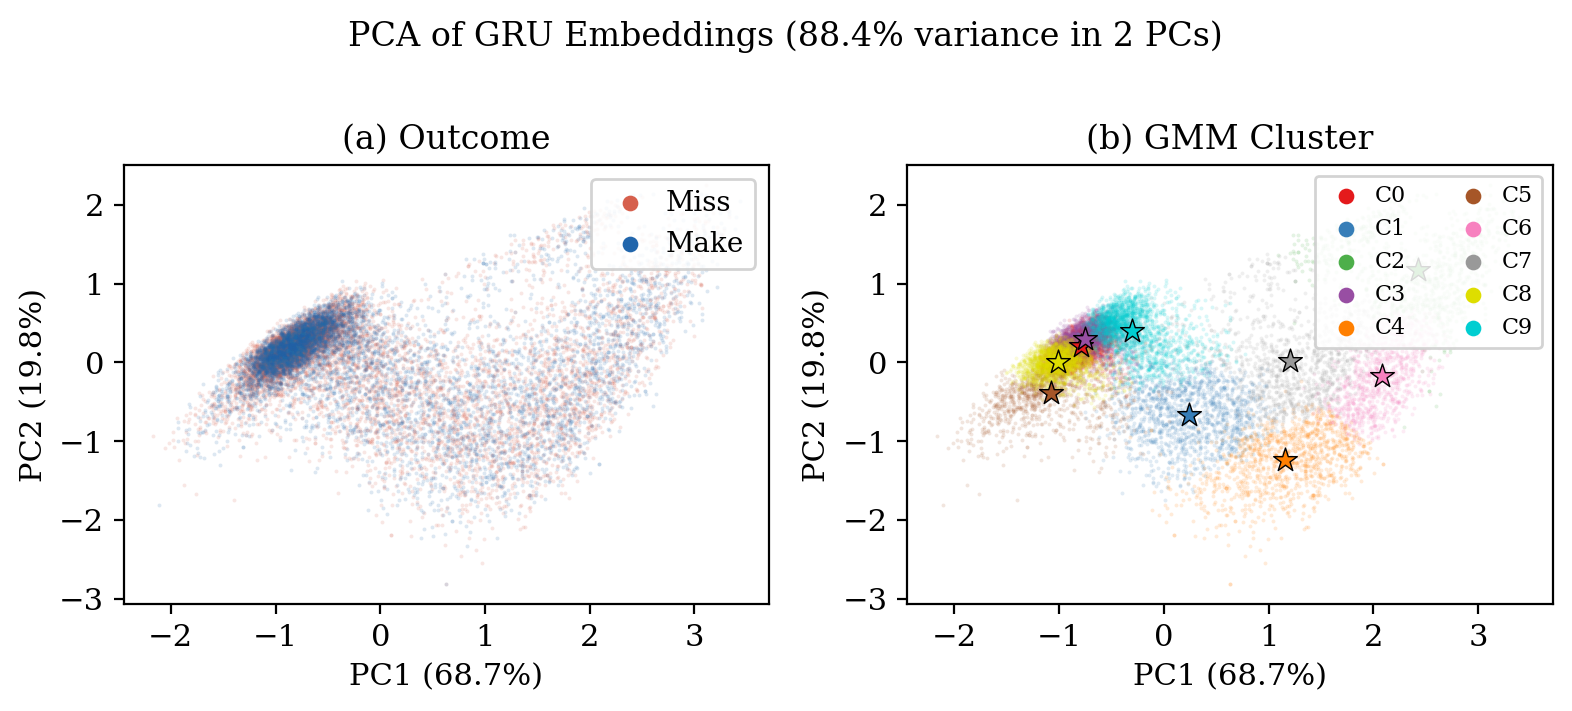
\includegraphics[width=0.62\linewidth]{pca_gmm_scatter.png}
      \vspace{-2ex}
      \caption{(a) PCA by outcome; (b) by GMM cluster.}
    \end{figure}
    \vspace{-2ex}
    \begin{table}
      \centering
      \scriptsize
      \begin{tabular}{c r c c c c l}
        \toprule
        \textbf{Cl.} & $n$ & \textbf{FG\%} & \textbf{Dist} & \textbf{\%3PT} & \textbf{Clock} & \textbf{Archetype} \\
        \midrule
        2 & 5,461 & 87.7 & 5.7 & 0.0 & 18.5 & At-rim / dunks \\
        6 & 5,415 & 65.2 & 2.7 & 0.0 & 15.9 & Putbacks \\
        7 & 6,049 & 62.0 & 5.8 & 0.7 & 13.9 & Short-range \\
        1 & 7,755 & 41.1 & 7.1 & 0.1 & 11.5 & Paint \\
        0 & 11,610 & 38.5 & 22.4 & 46.5 & 12.6 & Above-break 3s \\
        5 & 6,589 & 28.9 & 20.7 & 43.6 & 6.5 & Late-clock 3s \\
        \bottomrule
      \end{tabular}
      \vspace{-1ex}
      \caption{Selected GMM clusters ($K{=}10$). The GNN's latent space recovers recognizable shot archetypes.}
    \end{table}
  \end{block}

\end{column}

\separatorcolumn

% ============================================================
% COLUMN 3
% ============================================================
\begin{column}{\colwidth}

  \begin{block}{Results}
    \begin{table}
      \centering
      \small
      \begin{tabular}{l c c c}
        \toprule
        \textbf{Method} & \textbf{AUC} & \textbf{Acc} & \textbf{F1} \\
        \midrule
        \textbf{Static-38 + GMM} & \textbf{0.6551}$_{\pm.002}$ & \textbf{62.8\%} & \textbf{0.477} \\
        XGBoost Vel-65 & 0.6501$_{\pm.003}$ & 62.4\% & 0.476 \\
        XGBoost Static-38 & 0.6476$_{\pm.003}$ & 62.2\% & 0.476 \\
        TemporalGRU (GNN) & 0.6451 & 62.4\% & 0.445 \\
        LR Vel-65 Lasso & 0.6377$_{\pm.002}$ & 61.2\% & 0.520 \\
        Decision Tree d=7 & 0.6318$_{\pm.002}$ & 61.2\% & 0.436 \\
        \bottomrule
      \end{tabular}
      \vspace{-1ex}
      \caption{Top results (87,147 shots; 5-fold CV for baselines; 70/20/10 for GNN).}
    \end{table}
    \vspace{-2ex}
    \begin{figure}
      \centering
      \begin{minipage}{0.38\linewidth}
        \centering
        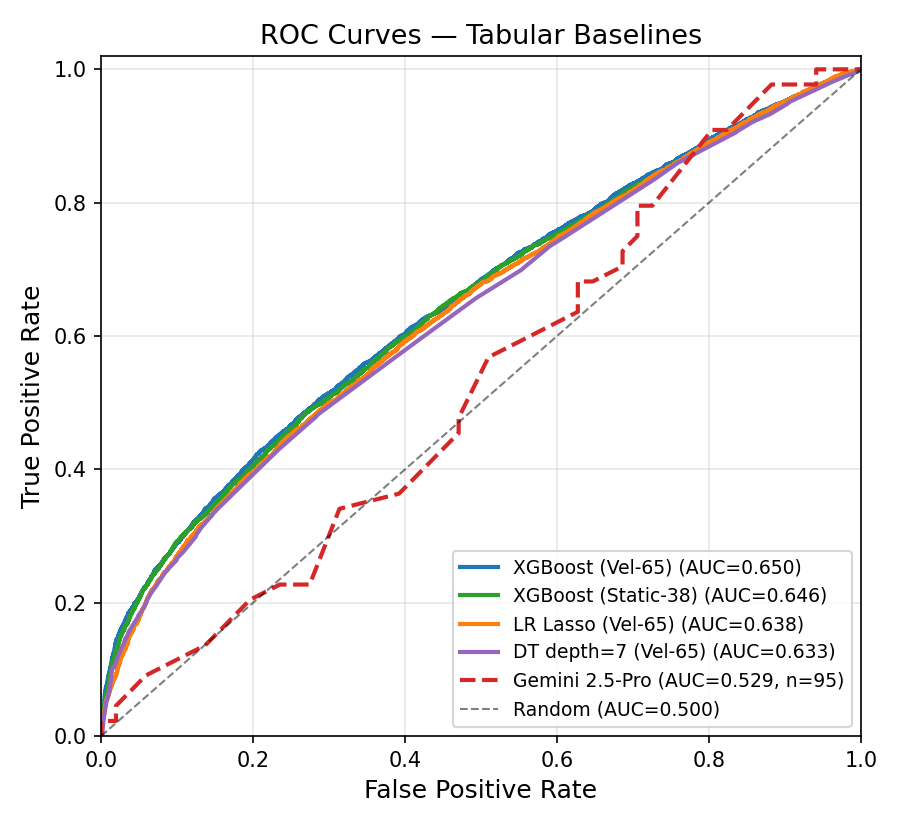
\includegraphics[width=\linewidth]{baseline_roc_curves.png}
      \end{minipage}\hfill
      \begin{minipage}{0.38\linewidth}
        \centering
        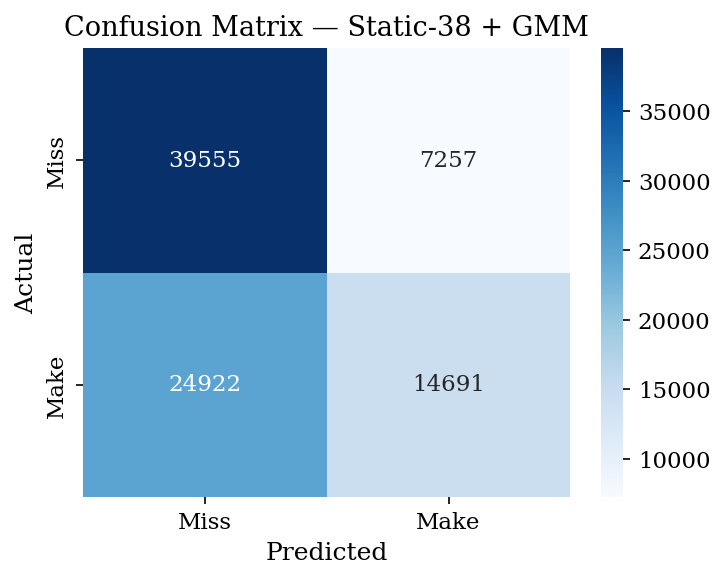
\includegraphics[width=\linewidth]{cm_Static_38_plus_GMM.png}
      \end{minipage}
      \vspace{-2ex}
      \caption{Baselines --- Left: ROC curves. Right: CM (Static-38 + GMM).}
    \end{figure}
    \vspace{-2.5ex}
    \begin{figure}
      \centering
      \begin{minipage}{0.38\linewidth}
        \centering
        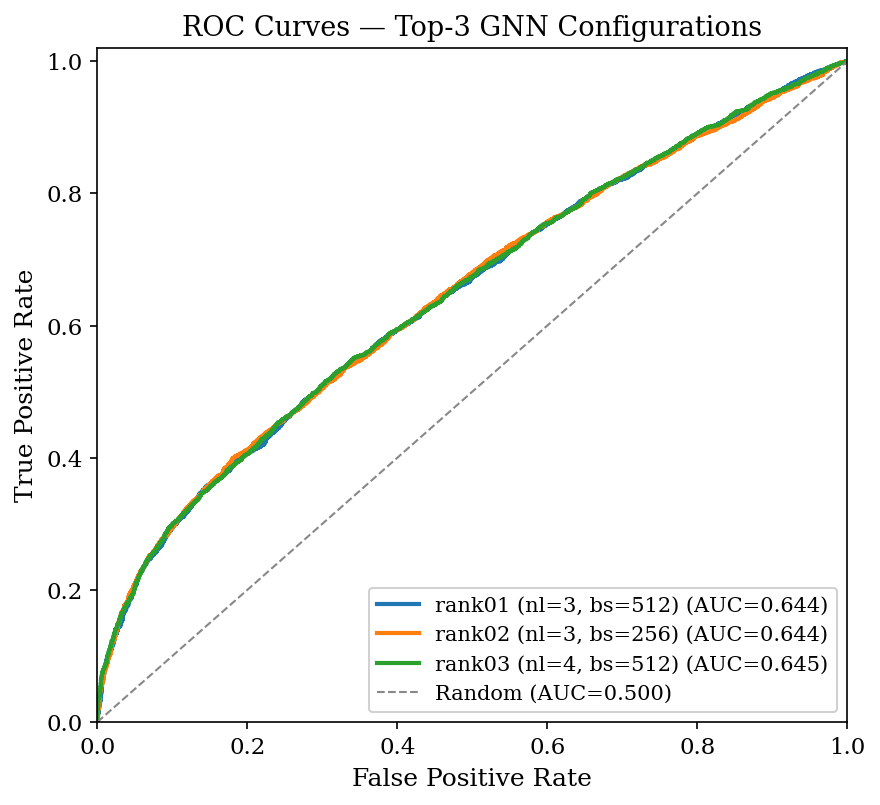
\includegraphics[width=\linewidth]{roc_curves_ranks.png}
      \end{minipage}\hfill
      \begin{minipage}{0.38\linewidth}
        \centering
        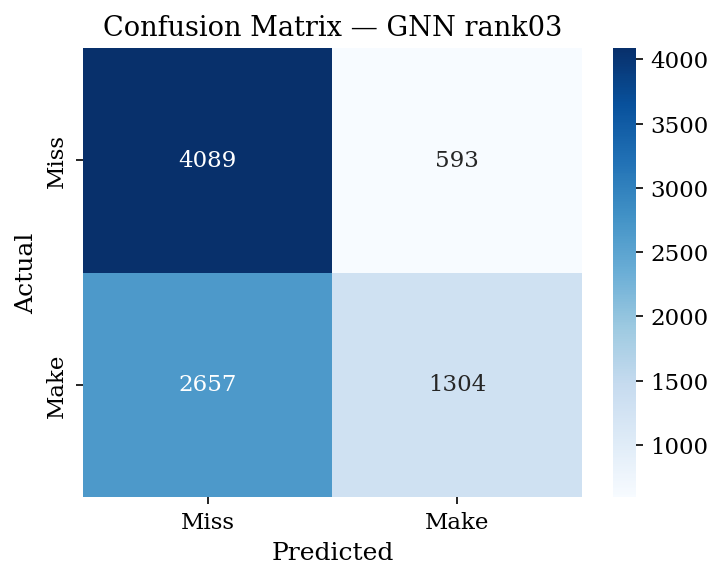
\includegraphics[width=\linewidth]{cm_gnn_rank03.png}
      \end{minipage}
      \vspace{-2ex}
      \caption{GNN --- Left: ROC for top-3 configs. Right: CM (TemporalGRU rank03).}
    \end{figure}
  \end{block}

  \begin{block}{Discussion}
    The hybrid succeeds because the GNN and XGBoost extract largely \textbf{orthogonal} signals: XGBoost relies on \textbf{shot distance and shooter FG\%}, while the GNN encodes \textbf{defender rotations, shot-creation dynamics, and court configuration}. Feature ablation confirms the GNN derives signal from \textit{how the shot is taken} ($\Delta$AUC for player stats $= -0.0018$, least important)---nearly the inverse of tabular baselines.
    Moderate AUC ($\sim$0.65) reflects basketball's inherent stochasticity (published: 0.59--0.65). HP tuning (+0.0105) $>$ architecture; data scaling (1.7K$\to$87K) was the dominant bottleneck.
  \end{block}

  \begin{block}{Future Work}
    With six more months: (1) replace GRU with a transformer encoder, extending context to 3--5\,s---our ablation shows a striking interaction effect for richer temporal context; (2) train on multi-season data (2013--16, $\sim$300K shots) for generalization and era-adjusted player evaluation; (3) build a real-time pipeline ingesting live SportVU feeds for coaching decisions and sports-betting calibration.
  \end{block}

  \vspace{-1ex}
  {\usebeamerfont{heading}\usebeamercolor[fg]{heading}References}\par\smallskip
  {\scriptsize
  [1] Chen, T.\ \& Guestrin, C.\ ``XGBoost: A Scalable Tree Boosting System.'' \textit{KDD}, 2016.\par
  [2] Brody, S.\ et al.\ ``How Attentive are Graph Attention Networks?'' \textit{ICLR}, 2022.\par
  [3] Cho, K.\ et al.\ ``Learning Phrase Representations using RNN Encoder-Decoder.'' \textit{EMNLP}, 2014.\par
  }

\end{column}

\separatorcolumn
\end{columns}
\end{frame}

\end{document}
